\documentclass{../myclass}
\usepackage[polish]{babel}

\begin{document}

\begin{center}
    \Large \textbf{Laboratorium 4.}\\
    \large
    \textsc{Permutacje macierzy}\\
    \normalsize
    Bartosz Hanc
\end{center}

\section{Wstęp}

Celem ćwiczenia było napisanie algorytmów permutacji macierzy: Minimum Degree, Cuthill--MacKee oraz
Reversed Cuthill-MacKee oraz zbadanie ich wpływu na kompresje macierzy rzadkich opisujących
topologię siatki trójwymiarowej zbudowanej z sześciennych komórek dla siatek o rozmiarach \(4\times
4\times 4\), \(8 \times 8 \times 8\) oraz \(16\times16\times16\). Wygenerowano również wizualizacje
uzyskanych po permutacji i kompresji macierzy hierarchicznych.

\section{Kod rozwiązania}

Poniżej zamieszczono kod rozwiązania w języku Python. Nieskierowany graf macierzy symetrycznej był
reprezentowany przez strukturę \pythoninline{Graph}, szczególności graf został opisany przez listę
sąsiedztwa (pole \pythoninline{Graph.adj}). Funkcje \pythoninline{MinimumDegree(G: Graph)},
\pythoninline{CuthillMacKee(G: Graph)} oraz \pythoninline{ReversedCuthillMcKee(G: Graph)}
implementujące odpowiednio algorytmy zwracają listę opisującą permutację macierzy wejściowej
reprezentowanej przez graf \pythoninline{G}. Macierze były reprezentowane jako dwuwymiarowe tablice
z biblioteki Numpy.

\begin{python}
class Graph:
    def __init__(self, A: np.ndarray):
        n = A.shape[0]
        self.adj = {u: {v for v in range(n) if A[u, v] > 0 and u != v} 
                    for u in range(n)}
\end{python}

\begin{python}
def MinimumDegree(G: Graph) -> np.ndarray:
    n = len(G.adj)
    order = []

    for _ in range(n):
        p = min(G.adj, key=lambda v: len(G.adj[v]))
        order.append(p)
        for u in G.adj[p]:
            G.adj[u] |= G.adj[p]
            G.adj[u] -= {p, u}
        del G.adj[p]

    return np.array(order)
\end{python}

\begin{python}
from collections import deque

def CuthillMcKee(G: Graph) -> np.ndarray:
    queue, order, visit = deque(), [], {v: False for v in G.adj}
    p = min(G.adj, key=lambda x: len(G.adj[x]))
    order.append(p)
    visit[p] = True

    for u in sorted(G.adj[p], key=lambda x: len(G.adj[x])):
        queue.append(u)

    while len(queue) > 0:
        u = queue.popleft()

        if not visit[u]:
            order.append(u)
            visit[u] = True

            for v in sorted(G.adj[u], key=lambda x: len(G.adj[x])):
                if not visit[v]: queue.append(v)

    return np.array(order)
\end{python}

\begin{python}
def ReversedCuthillMcKee(G: Graph) -> np.ndarray:
    return CuthillMcKee(G)[::-1]
\end{python}

Mając daną listę \pythoninline{order} opisującą permutację macierzy zwróconą przez jeden z powyższych algorytmów samą permutację macierzy \pythoninline{A} można wykonać jako
\begin{python}
A = A[order, :][:, order]
\end{python}

\section{Wyniki}

Zgodnie z poleceniem wygenerowano losowe macierze o strukturze opisującej topologię siatek
trójwymiarowych o komórkach sześciennych rozmiarów \(4\times 4\times 4\), \(8 \times 8 \times 8\)
oraz \(16\times16\times16\). Poniżej na Rysunku \ref{Fig:1} zamieszczono wzorce rzadkości tych
macierzy oraz uzyskaną przez kompresję macierz hierarchiczną przed zastosowaniem permutacji.

\begin{figure}
    \centering
    \begin{subfigure}[b]{0.45\textwidth}
        \centering
        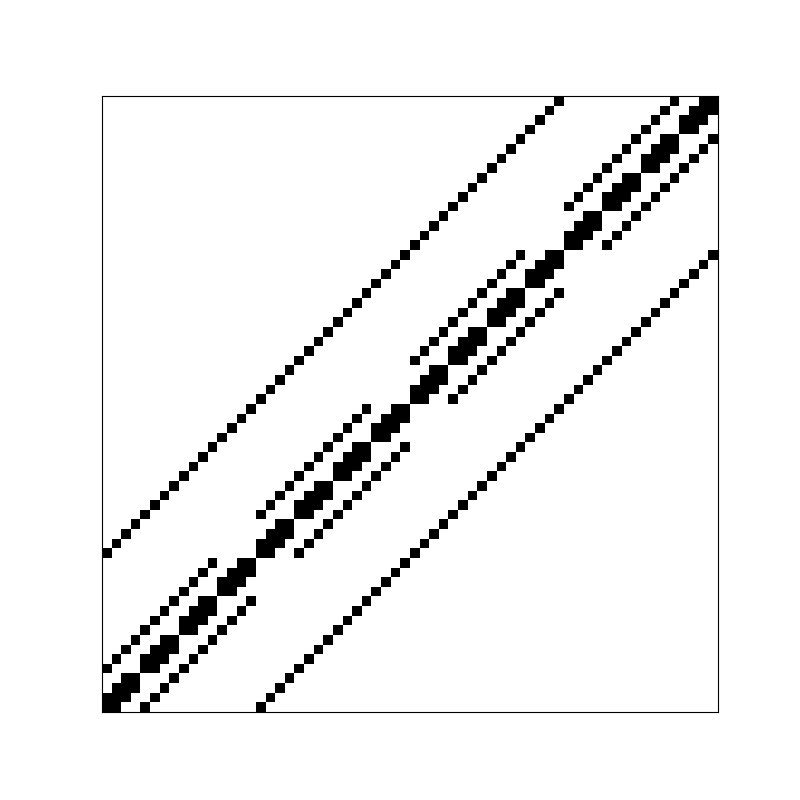
\includegraphics[width=\textwidth]{0_bp_sp.png}
    \end{subfigure}
    \hfill
    \begin{subfigure}[b]{0.45\textwidth}
        \centering
        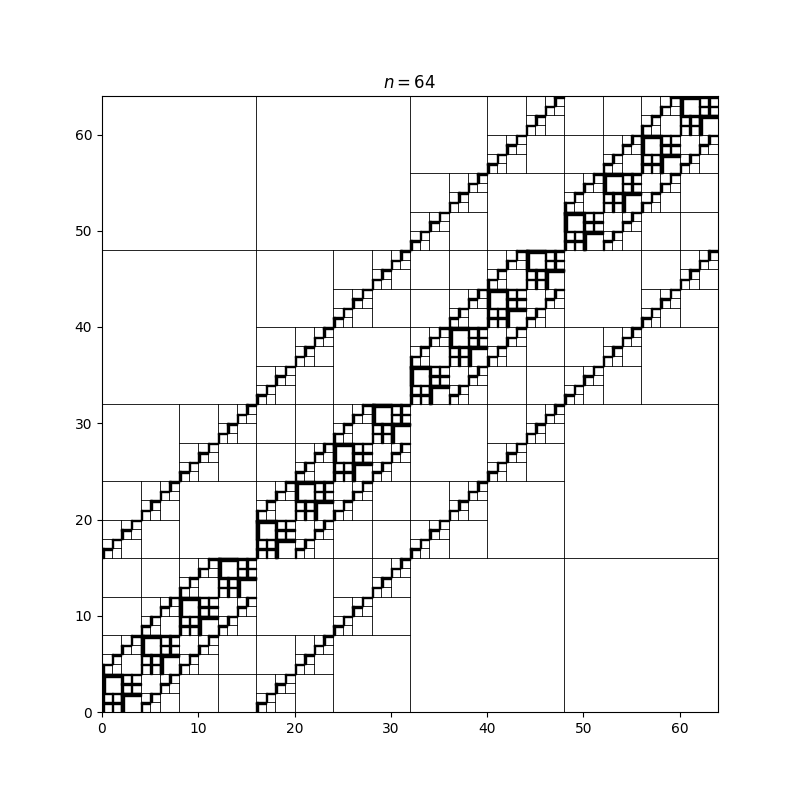
\includegraphics[width=\textwidth]{0_bp_hm.png}
    \end{subfigure}
    \vfill
    \centering
    \begin{subfigure}[b]{0.45\textwidth}
        \centering
        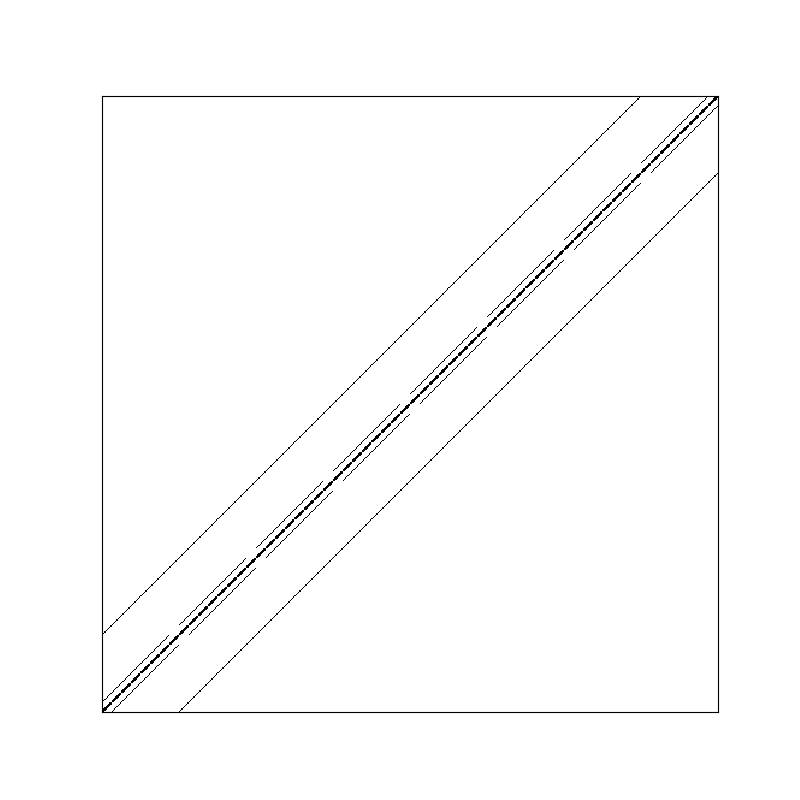
\includegraphics[width=\textwidth]{1_bp_sp.png}
    \end{subfigure}
    \hfill
    \begin{subfigure}[b]{0.45\textwidth}
        \centering
        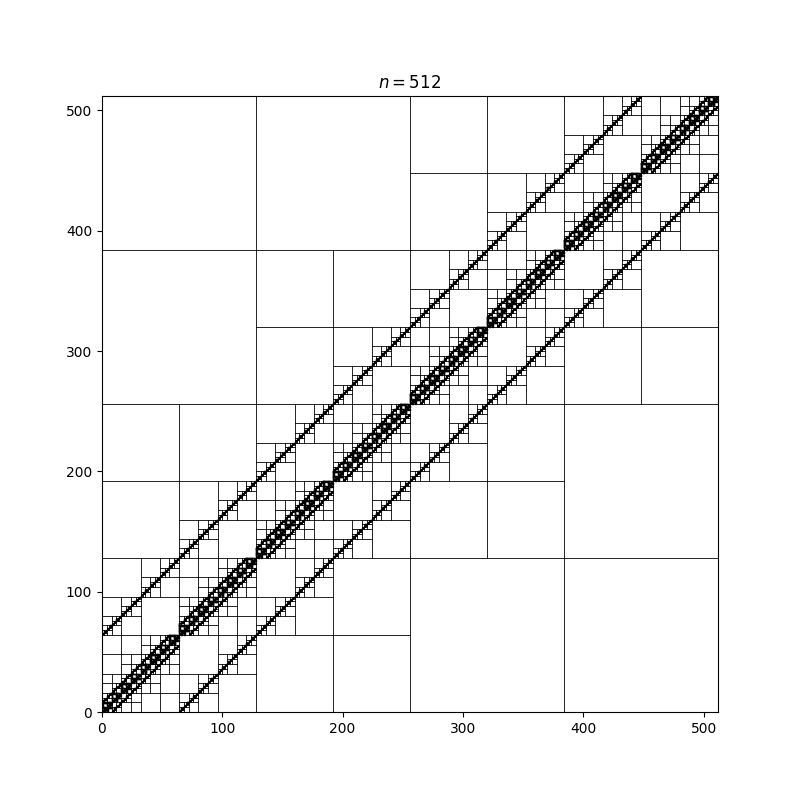
\includegraphics[width=\textwidth]{1_bp_hm.png}
    \end{subfigure}
    \vfill
    \centering
    \begin{subfigure}[b]{0.45\textwidth}
        \centering
        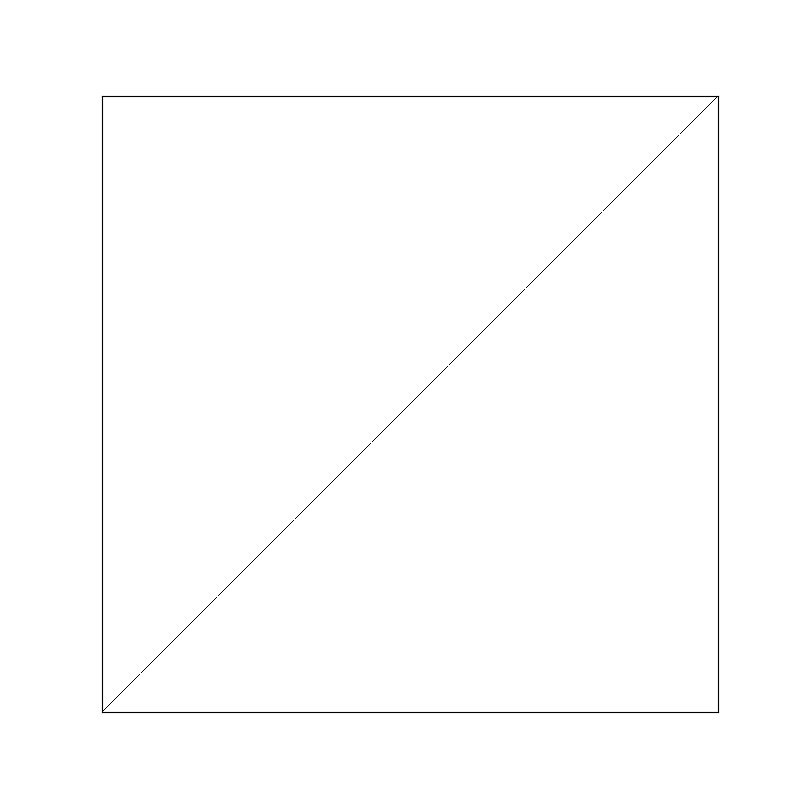
\includegraphics[width=\textwidth]{2_bp_sp.png}
    \end{subfigure}
    \hfill
    \begin{subfigure}[b]{0.45\textwidth}
        \centering
        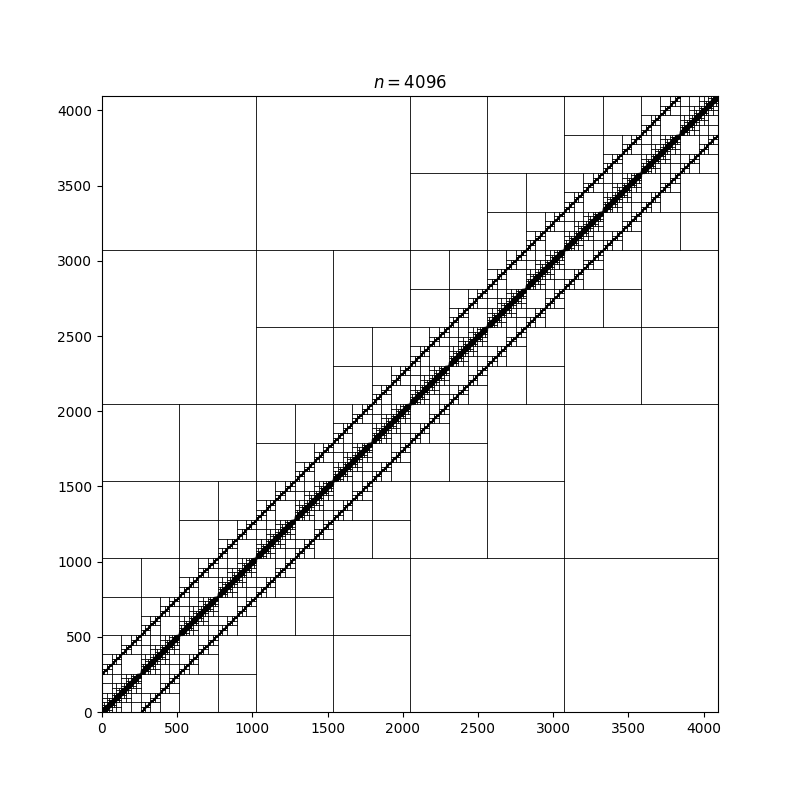
\includegraphics[width=\textwidth]{2_bp_hm.png}
    \end{subfigure}
    \caption{Wzorce rzadkości oraz uzyskane macierze hierarchiczne dla macierzy wejściowych przed permutacją}
    \label{Fig:1}
\end{figure}

\begin{figure}
    \centering
    \begin{subfigure}[b]{0.45\textwidth}
        \centering
        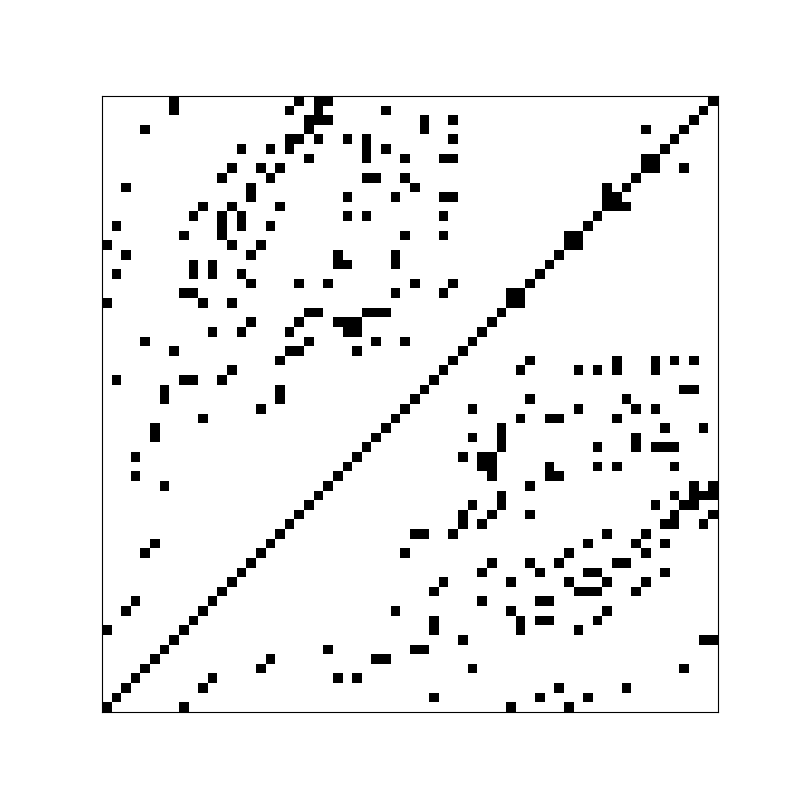
\includegraphics[width=\textwidth]{0_ap_sp_mindeg.png}
    \end{subfigure}
    \hfill
    \begin{subfigure}[b]{0.45\textwidth}
        \centering
        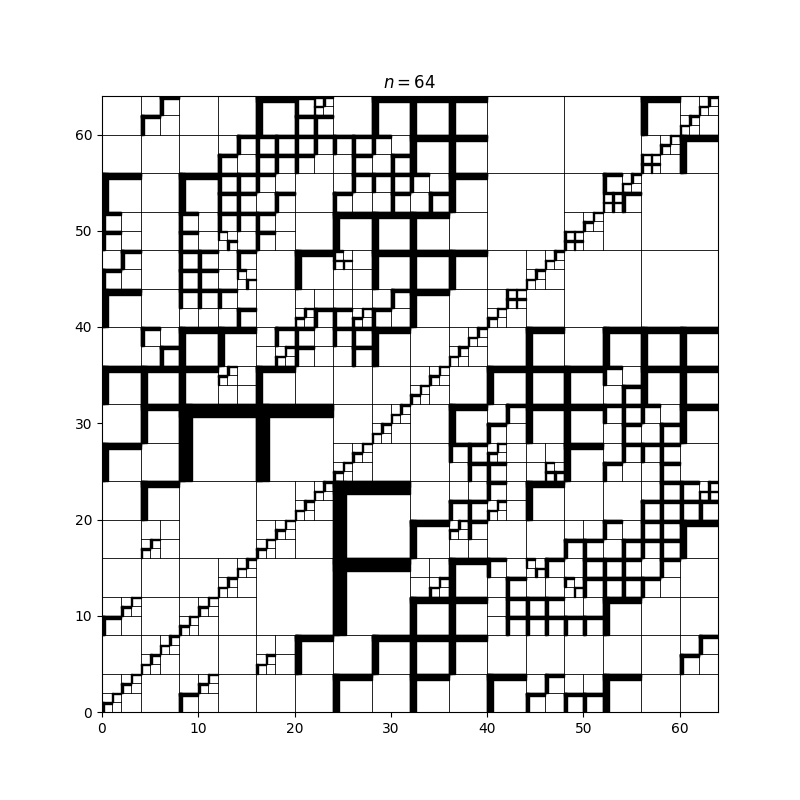
\includegraphics[width=\textwidth]{0_ap_hm_mindeg.png}
    \end{subfigure}
    \vfill
    \centering
    \begin{subfigure}[b]{0.45\textwidth}
        \centering
        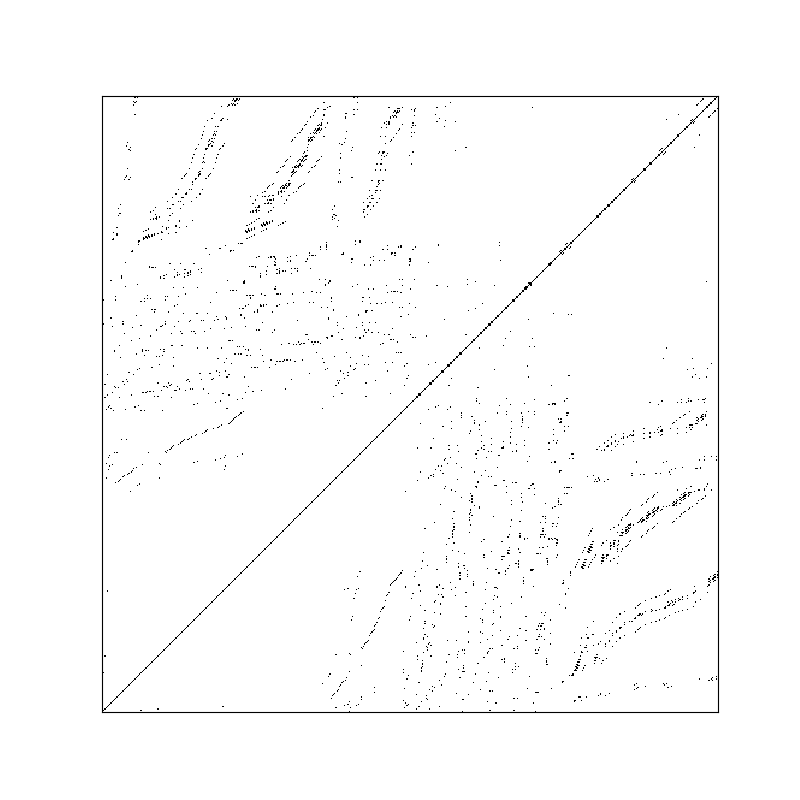
\includegraphics[width=\textwidth]{1_ap_sp_mindeg.png}
    \end{subfigure}
    \hfill
    \begin{subfigure}[b]{0.45\textwidth}
        \centering
        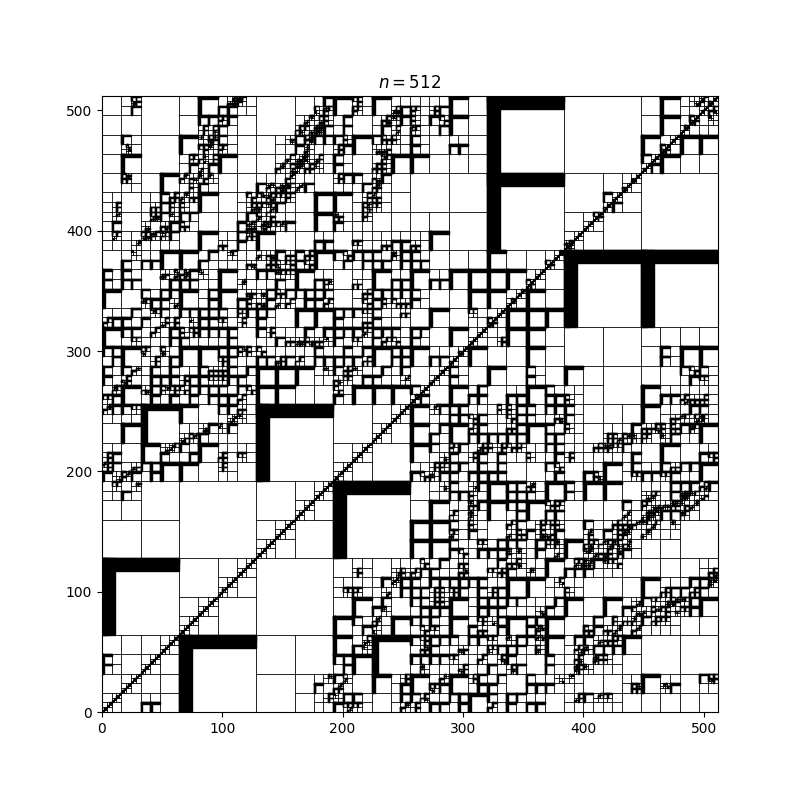
\includegraphics[width=\textwidth]{1_ap_hm_mindeg.png}
    \end{subfigure}
    \vfill
    \centering
    \begin{subfigure}[b]{0.45\textwidth}
        \centering
        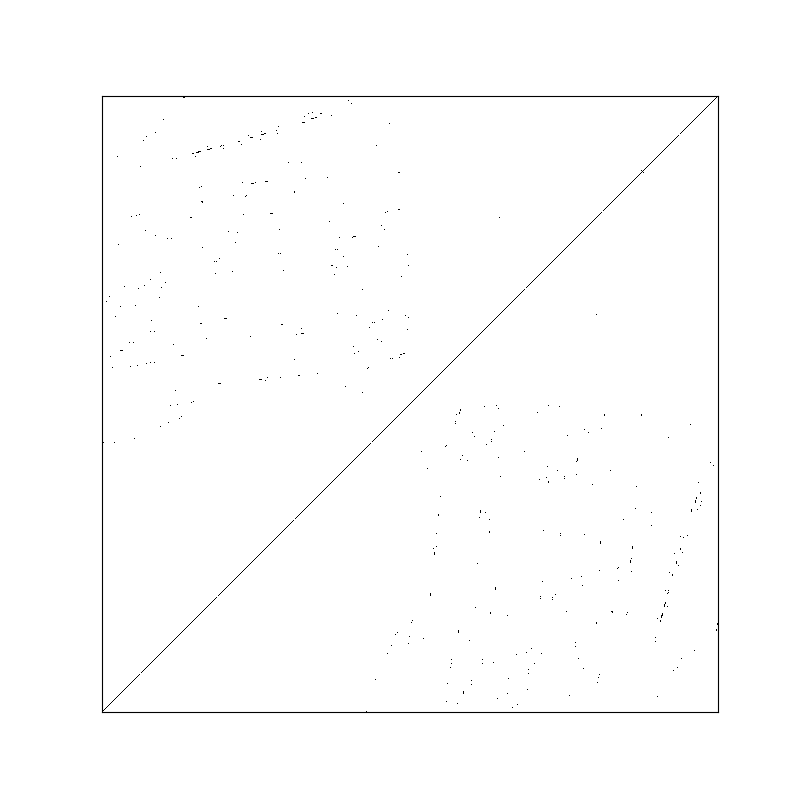
\includegraphics[width=\textwidth]{2_ap_sp_mindeg.png}
    \end{subfigure}
    \hfill
    \begin{subfigure}[b]{0.45\textwidth}
        \centering
        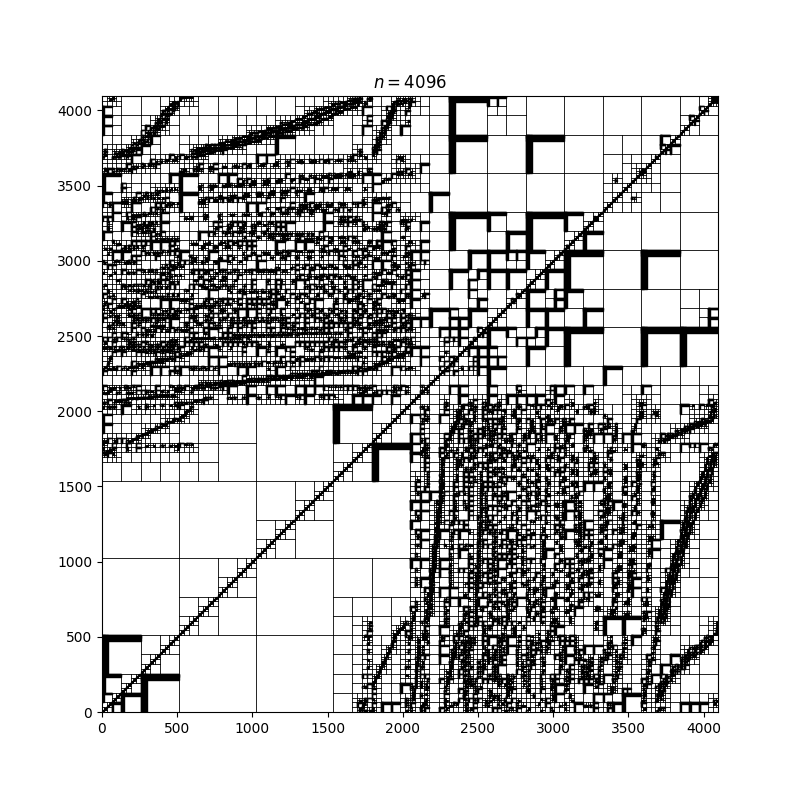
\includegraphics[width=\textwidth]{2_ap_hm_mindeg.png}
    \end{subfigure}
    \caption{Wzorce rzadkości oraz uzyskane macierze hierarchiczne dla macierzy wejściowych po permutacji korzystającej z algorytmu Minimum Degree}
    \label{Fig:2}
\end{figure}

\begin{figure}
    \centering
    \begin{subfigure}[b]{0.45\textwidth}
        \centering
        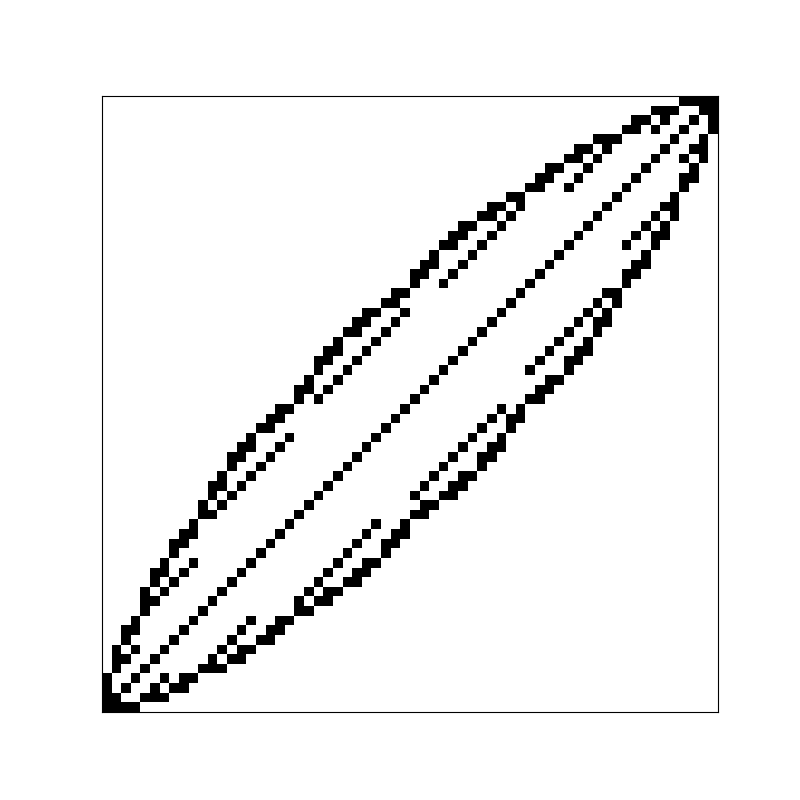
\includegraphics[width=\textwidth]{0_ap_sp_cutkee.png}
    \end{subfigure}
    \hfill
    \begin{subfigure}[b]{0.45\textwidth}
        \centering
        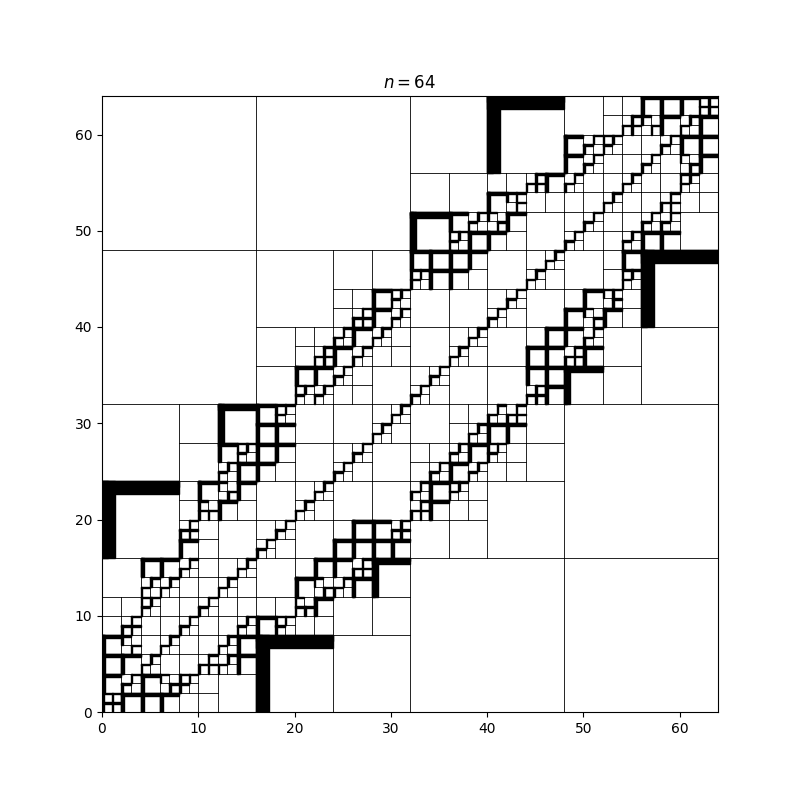
\includegraphics[width=\textwidth]{0_ap_hm_cutkee.png}
    \end{subfigure}
    \vfill
    \centering
    \begin{subfigure}[b]{0.45\textwidth}
        \centering
        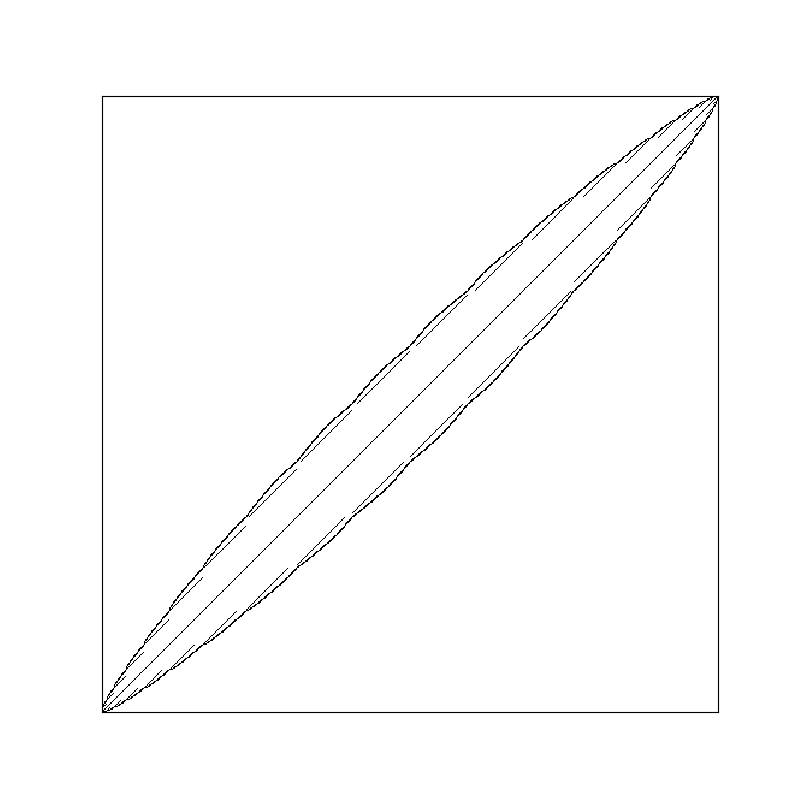
\includegraphics[width=\textwidth]{1_ap_sp_cutkee.png}
    \end{subfigure}
    \hfill
    \begin{subfigure}[b]{0.45\textwidth}
        \centering
        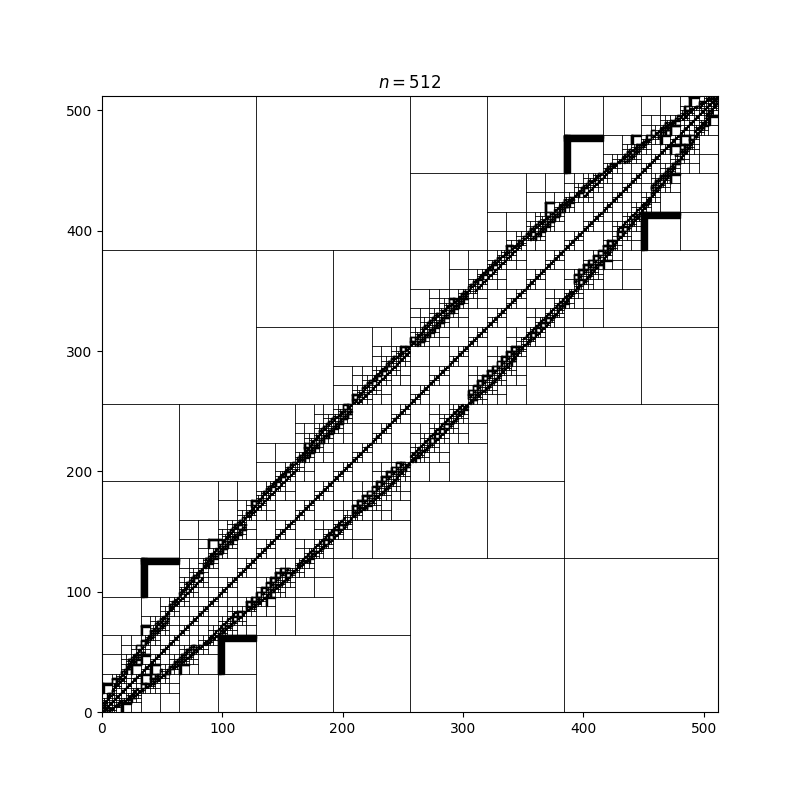
\includegraphics[width=\textwidth]{1_ap_hm_cutkee.png}
    \end{subfigure}
    \vfill
    \centering
    \begin{subfigure}[b]{0.45\textwidth}
        \centering
        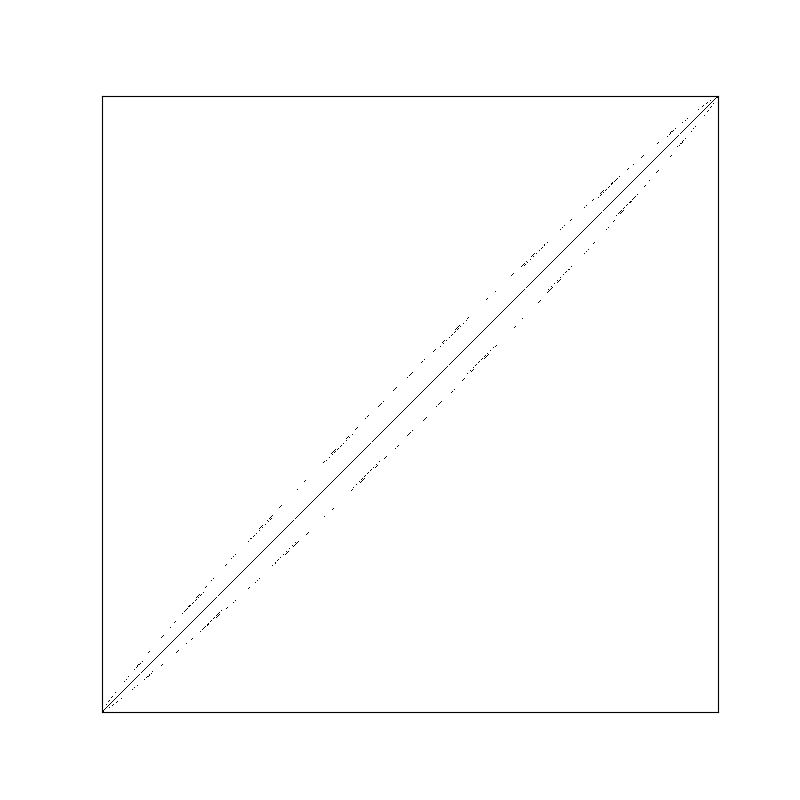
\includegraphics[width=\textwidth]{2_ap_sp_cutkee.png}
    \end{subfigure}
    \hfill
    \begin{subfigure}[b]{0.45\textwidth}
        \centering
        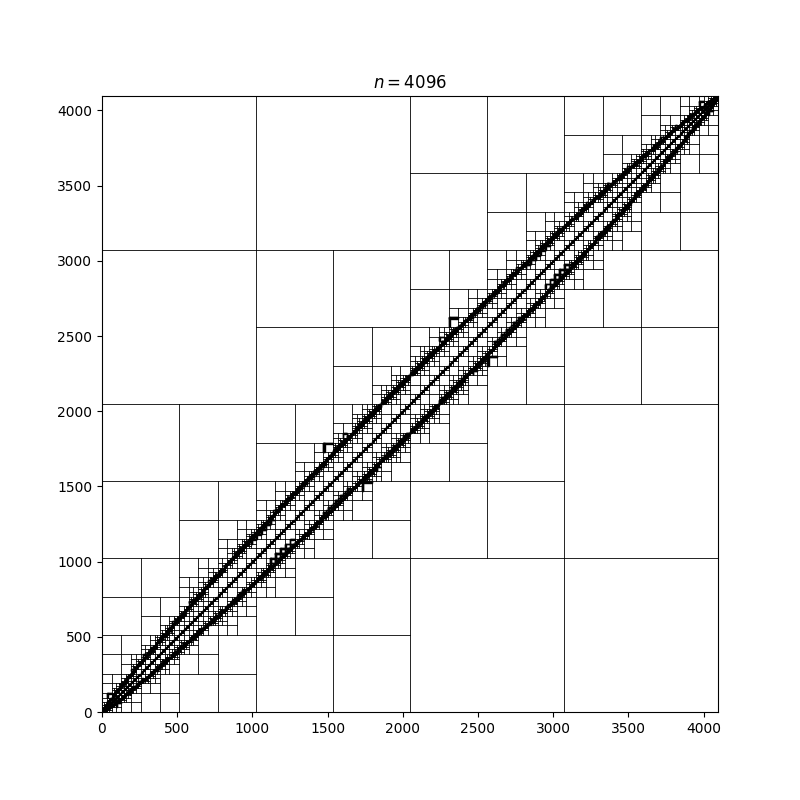
\includegraphics[width=\textwidth]{2_ap_hm_cutkee.png}
    \end{subfigure}
    \caption{Wzorce rzadkości oraz uzyskane macierze hierarchiczne dla macierzy wejściowych po permutacji korzystającej z algorytmu Cuthill--MacKee}
    \label{Fig:3}
\end{figure}

\end{document}